\documentclass[12pt,a4paper]{article}
\usepackage[utf8]{inputenc}
\usepackage[T1]{fontenc}
\usepackage{fontspec}
\usepackage[polish]{babel}
\usepackage{amsmath}
\usepackage{graphicx}
\usepackage[table,xcdraw]{xcolor}
\usepackage{hhline}
\usepackage{placeins}
\usepackage[margin=0.6in]{geometry}
\usepackage{appendix}
\usepackage{colortbl}
\usepackage{physics}
\usepackage{float}
\usepackage{datetime}
\usepackage{hyperref}

\title{Praca Domowa Termodynamika i Fizyka Statystyczna R 2021/2022}
\author{Kacper Cybiński}
% \newdate{date}{28}{01}{2022}
% \date{\displaydate{date}}
\date{\today}
\setlength\parindent{0pt}

\newcommand{\com}[1]{{\color{red} #1}}

\newcommand{\link}[2]{{\color{cyan} \href{#1}{#2}}}

\renewcommand{\emph}{\textbf}

\begin{document}

\maketitle

\section{Zadanie 3}

\begin{figure}[h!]
    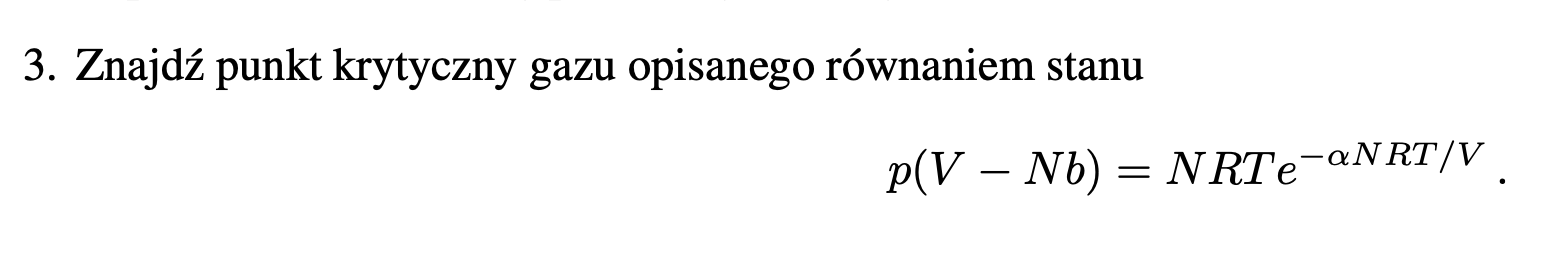
\includegraphics[width=\linewidth]{z3.png}
\end{figure}

\section{Rozwiązanie}

Rozpatrywany gaz opisany jest równaniem stanu postaci:
$$
p(V-N b)=N R T \exp \left(-\frac{\alpha N R T}{V}\right)
$$
Stąd ciśnienie gazu dane jest wzorem:
$$
p=\frac{N R T \exp \left(-\frac{\alpha N R T}{V}\right)}{V-N b}
$$
Punkt krytyczny gazu, to takie wartości $V_{k r}, T_{k r}, p_{k r}$, dla których zachodzą równania:
$$
\begin{aligned}
&\left(\frac{\partial p}{\partial T}\right)_{V}=0 \\
&\left(\frac{\partial^{2} p}{\partial^{2} T}\right)_{V}=0
\end{aligned}
$$
Obliczając pochodne dostajemy układ równań:
$$
\frac{N R T e^{-\frac{\alpha N R T}{V}}\left(\alpha N R T(b N-V)+V^{2}\right)}{V^{2}(V-b N)^{2}}=0
$$
$-\frac{N R T e^{-\frac{\alpha N R T}{V}}\left(\alpha^{2} N^{2} R^{2} T^{2}(V-b N)^{2}-2 \alpha N R T V\left(b^{2} N^{2}-3 b N V+2 V^{2}\right)+2 V^{4}\right)}{V^{4}(b N-V)^{3}}=0$
A stąd dostajemy, że równania te spełnione są dla $V_{k r}=2 b N$ i $T_{k r}=\frac{4 b}{\alpha R}$, natomiast $p_{k r}$ jest równe $p_{k r}=\frac{4}{\alpha e^{2}}$


\end{document}